\documentclass[preprint,12pt]{elsarticle}
\usepackage[T1]{fontenc}
\usepackage{lmodern}
\usepackage{amsmath,amssymb,amsthm}
\usepackage{graphicx}
\usepackage{booktabs}
\usepackage{multirow}
\usepackage{adjustbox}
\usepackage{microtype}
\usepackage[section]{placeins}
\usepackage{xr}
\externaldocument{main}
\usepackage{xcolor}
\usepackage{fvextra}
\usepackage[capitalise,nameinlink]{cleveref}
\setlength{\emergencystretch}{2em}
\renewcommand{\thesection}{S\arabic{section}}
\renewcommand{\thetable}{S\arabic{table}}
\renewcommand{\thefigure}{S\arabic{figure}}
\renewcommand{\theequation}{S\arabic{equation}}
\newtheorem{assumption}{Assumption}
\newcommand{\supp}[1]{Section~S#1}
\journal{Image and Vision Computing}
\begin{document}
\begin{frontmatter}
\title{Supplementary material for ``CARA: Conformally calibrated, drift-aware rotation averaging for global structure-from-motion''}
\author[a]{Siva Ramakrishna Jeevakala}
\author[b]{A. P. Siva Kumar}
\affiliation[a]{organization={Department of Computer Science and Engineering (AI \& ML), G. Pulla Reddy Engineering College (Autonomous)}, city={Kurnool}, postcode={518007}, state={Andhra Pradesh}, country={India}}
\affiliation[b]{organization={Department of Computer Science and Engineering, JNTUA College of Engineering, Jawaharlal Nehru Technological University Anantapur}, city={Ananthapuramu}, postcode={515002}, state={Andhra Pradesh}, country={India}}
\end{frontmatter}

References to numbered sections, tables, figures, equations and results without the prefix S point to the main paper.



\section{First ETH3D run (fixed split)}\label{sec:eth3d1}
This experiment removes the two main gaps of the synthetic and Notre Dame experiments of the main paper: the relative rotations and their uncertainty come from a learned network run on real images, and the degradations act on pixels, not on rotations.

\paragraph{Protocol} We use the 13 scenes of the ETH3D high-resolution multi-view training set~\cite{schops2017eth3d}, split by scene before any result was seen: 6 scenes for calibration (electro, kicker, meadow, pipes, relief\_2, terrains) and 7 for testing (courtyard, delivery\_area, facade, office, playground, relief, terrace), so calibration and test share no image and no place. Each sub-scene is a random set of 12 images; the view graph links each image to its 6 nearest cameras by viewing direction and position (on average 38.6 edges). VGGT-1B~\cite{wang2025vggt} is run on every image pair (inputs downscaled to at most 1024\,px, then to VGGT's 518\,px), and the relative rotation is read from its camera head. The edge uncertainty is pre-registered as $\hat\sigma_{ij}=1/\mathrm{median}$ of VGGT's depth confidence over both images. Calibration uses 144 clean sub-scenes (24 per scene; 140 go to the four splits, reshuffled for each of 5 seeds). Each test scene has 10 sub-scenes under 7 conditions: clean; fog rendered with the atmospheric scattering model at median transmission $t\in\{0.7,0.5,0.3\}$, using depth predicted by VGGT on the clean image; low light (Poisson--Gaussian noise at $0.3$ and $0.15$ of the linear exposure); and synthetic rain streaks (490 test graphs). Sub-scenes with a disconnected view graph (4 of 70 per condition) are reduced to their largest component for every method. Edges with error above $5^\circ$ count as outliers; they are 22.4\% of clean test edges and 24--29\% under degradation, and 14--19\% of edges exceed $30^\circ$. Methods, configuration and metrics are those of Section~\ref{sec:protocol} of the main paper; ConfW now uses VGGT's confidence. Seeds only reshuffle the calibration splits, so the unit of inference is the test scene: we average over seeds and sub-scenes per scene and use an exact sign-flip test over the 7 scenes (smallest two-sided $p=1/64$).

\begin{table*}[!htbp]\centering\footnotesize
\caption{ETH3D with the VGGT front end: AUC@5$^\circ$ (mean over the 7 held-out test scenes, 95\% bootstrap interval over scenes; 70 sub-scenes of 12 cameras per condition, 5 calibration seeds). Best mean per row in bold. The last column counts test scenes on which CARA beats CG.}\label{tab:eth3d}
\setlength{\tabcolsep}{3pt}\resizebox{\textwidth}{!}{\begin{tabular}{lcccccccc}\toprule
Condition & CG & ConfW & GLOMAP-RA & Shonan-H & CG-$\hat\rho$ & CARA-static & CARA & CARA$>$CG \\\midrule
clean & 0.621\,{\scriptsize[0.501,0.731]} & 0.654\,{\scriptsize[0.538,0.757]} & 0.626\,{\scriptsize[0.513,0.738]} & 0.589\,{\scriptsize[0.465,0.701]} & 0.628\,{\scriptsize[0.504,0.739]} & \textbf{0.657\,{\scriptsize[0.558,0.735]}} & 0.648\,{\scriptsize[0.538,0.736]} & 3/7 \\
fog $t{=}0.7$ & 0.609\,{\scriptsize[0.484,0.726]} & \textbf{0.640\,{\scriptsize[0.509,0.759]}} & 0.612\,{\scriptsize[0.491,0.729]} & 0.571\,{\scriptsize[0.453,0.687]} & 0.608\,{\scriptsize[0.475,0.730]} & 0.626\,{\scriptsize[0.499,0.736]} & 0.622\,{\scriptsize[0.496,0.733]} & 3/7 \\
fog $t{=}0.5$ & 0.596\,{\scriptsize[0.470,0.716]} & \textbf{0.653\,{\scriptsize[0.533,0.757]}} & 0.594\,{\scriptsize[0.463,0.717]} & 0.545\,{\scriptsize[0.412,0.671]} & 0.593\,{\scriptsize[0.465,0.716]} & 0.618\,{\scriptsize[0.503,0.722]} & 0.613\,{\scriptsize[0.500,0.722]} & 4/7 \\
fog $t{=}0.3$ & 0.569\,{\scriptsize[0.423,0.703]} & \textbf{0.601\,{\scriptsize[0.435,0.739]}} & 0.553\,{\scriptsize[0.389,0.702]} & 0.523\,{\scriptsize[0.372,0.661]} & 0.572\,{\scriptsize[0.435,0.700]} & 0.580\,{\scriptsize[0.449,0.694]} & 0.574\,{\scriptsize[0.427,0.701]} & 4/7 \\
low light $0.3$ & 0.544\,{\scriptsize[0.404,0.677]} & 0.565\,{\scriptsize[0.417,0.706]} & 0.564\,{\scriptsize[0.434,0.682]} & 0.536\,{\scriptsize[0.416,0.659]} & 0.570\,{\scriptsize[0.438,0.692]} & \textbf{0.581\,{\scriptsize[0.444,0.702]}} & 0.565\,{\scriptsize[0.412,0.697]} & 3/7 \\
low light $0.15$ & 0.502\,{\scriptsize[0.355,0.656]} & 0.546\,{\scriptsize[0.387,0.686]} & 0.526\,{\scriptsize[0.395,0.657]} & 0.491\,{\scriptsize[0.350,0.625]} & 0.497\,{\scriptsize[0.353,0.645]} & \textbf{0.584\,{\scriptsize[0.458,0.697]}} & 0.571\,{\scriptsize[0.441,0.689]} & 6/7 \\
rain & 0.528\,{\scriptsize[0.427,0.629]} & 0.524\,{\scriptsize[0.422,0.634]} & 0.512\,{\scriptsize[0.411,0.625]} & 0.505\,{\scriptsize[0.408,0.613]} & 0.528\,{\scriptsize[0.422,0.633]} & 0.534\,{\scriptsize[0.427,0.635]} & \textbf{0.546\,{\scriptsize[0.444,0.646]}} & 3/7 \\
\bottomrule\end{tabular}}\end{table*}


\paragraph{What the degradations do to VGGT} VGGT is robust to these degradations. From clean to the strongest fog and low light, the median error of inlier edges grows only from $0.70^\circ$ to $0.75^\circ$ and $0.85^\circ$ (rain: $1.32^\circ$), while the fraction of edges above $30^\circ$ grows from 14.1\% to 16.7\% and 19.2\%. The shift is therefore mainly more gross failures, not a rescaling of inlier noise, which is the case Assumption~\ref{ass:scale} of the main paper does not cover.

\paragraph{Accuracy} \Cref{tab:eth3d} and \cref{fig:eth3d}(a) report AUC@5$^\circ$. CARA's mean is above CG, GLOMAP-RA and Shonan-H in all seven conditions (by $0.005$--$0.069$ over CG, largest under low light at $0.15$), but the per-scene intervals overlap and CARA beats CG on only 3 to 6 of the 7 test scenes depending on the condition. Pooled over conditions the difference to CG is $+0.024$ (3 of 7 scenes, $p=0.47$) and to GLOMAP-RA $+0.022$ ($p=0.50$); only Shonan-H is beaten consistently (6 of 7 scenes, $p=0.047$, Holm-adjusted $0.23$). None of these differences is significant. ConfW, which only weights CG by VGGT's confidence, is as accurate as CARA (pooled difference $-0.006$) and has the lowest catastrophic rate in four of seven conditions; CARA's gates reject 60--80\% of outlier edges but also 8--10\% of inliers, and on 12-camera graphs this removes support that weighting keeps. CARA-static is within $0.016$ of CARA in every condition and slightly higher in six of seven, so the drift factor does not improve accuracy here, as expected when the inlier noise barely changes.

\begin{table}[!htbp]\centering\footnotesize
\caption{ETH3D with VGGT: per-camera bounds at target $1-\alpha_{\mathrm{cam}}=0.9$ (mean over test scenes, 95\% interval over scenes), median $\hat\rho$, and the ratio of the median inlier edge error to its clean value.}\label{tab:eth3dbounds}
\setlength{\tabcolsep}{2.5pt}\begin{adjustbox}{max width=\textwidth}\begin{tabular}{lcccccc}\toprule
 & \multicolumn{2}{c}{CARA} & \multicolumn{2}{c}{CARA-static} & & \\\cmidrule(lr){2-3}\cmidrule(lr){4-5}
Condition & cov. & hard & cov. & hard & $\hat\rho$ & ratio \\\midrule
clean & 0.886 & 0.760 & 0.887 & 0.774 & 1.00 & 1.00 \\
fog $t{=}0.7$ & 0.843 & 0.721 & 0.827 & 0.710 & 1.13 & 0.97 \\
fog $t{=}0.5$ & 0.841 & 0.737 & 0.832 & 0.751 & 1.11 & 0.99 \\
fog $t{=}0.3$ & 0.789 & 0.681 & 0.800 & 0.690 & 1.37 & 1.07 \\
low light $0.3$ & 0.812 & 0.691 & 0.813 & 0.709 & 1.24 & 1.13 \\
low light $0.15$ & 0.823 & 0.698 & 0.806 & 0.691 & 1.44 & 1.21 \\
rain & 0.852 & 0.717 & 0.810 & 0.678 & 1.42 & 1.89 \\
\bottomrule\end{tabular}\end{adjustbox}\end{table}


\paragraph{Per-camera bounds} On clean held-out scenes the calibrated bounds cover 88.6\% of registered cameras (95\% interval $[82.2,94.5]$\%) at a 90\% target (\cref{tab:eth3dbounds}, \cref{fig:eth3d}(b)). This is the first test of the guarantee with a learned front end, calibration and test on different places, and a real uncertainty proxy, and the result is consistent with the target. Under degradation, coverage falls to 78.9--85.2\%, and to 68--74\% on the quarter of cameras with the largest $u_i$. The drift factor responds ($\hat\rho$ median $1.1$--$1.4$ under shift, $1.0$ on clean scenes) and raises coverage over CARA-static by 1--4 points under rain ($85.2$ vs $81.0$\%), fog $0.7$, fog $0.5$ and low light $0.15$, but not under fog $0.3$ or low light $0.3$. A scalar noise factor cannot account for a higher rate of gross failures, so these bounds are optimistic by about 5--11 points under real shift.

\begin{figure}[!htbp]\centering
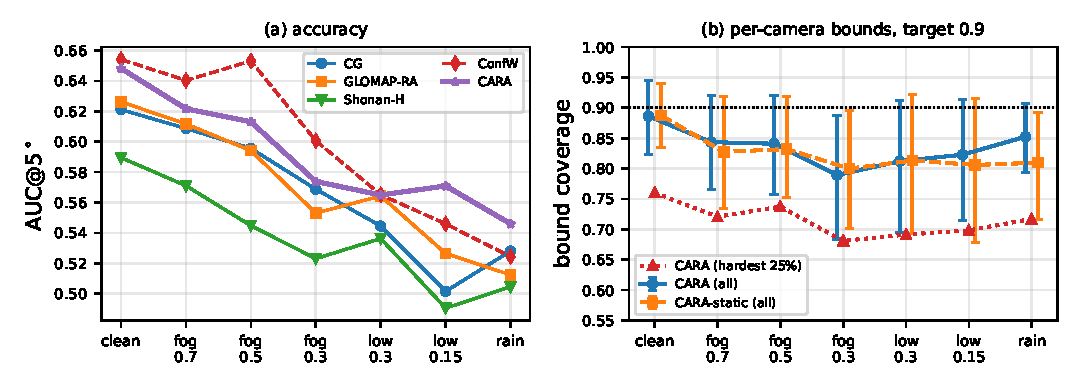
\includegraphics[width=\columnwidth]{figs/eth3d.pdf}
\caption{ETH3D with VGGT. (a) AUC@5$^\circ$ per condition (mean over 7 test scenes). (b) Coverage of the 90\% per-camera bounds with 95\% intervals over test scenes, and coverage on the hardest quarter of cameras; dotted line: target.}\label{fig:eth3d}
\end{figure}

\paragraph{Choice of confidence aggregate} VGGT's depth confidence has a floor of $1$, and for 55\% of edges the median over both images sits on it, so the pre-registered $\hat\sigma$ is constant on most edges. The pre-registered alternative, the exponential of the negative mean log-confidence, separates outlier edges much better (AUROC $0.89$ vs $0.73$ on clean test edges; Spearman correlation with error $-0.69$ vs $-0.44$). With it CARA's AUC@5 rises by $0.01$ on average ($0$ to $0.018$ per condition) (pooled difference to CG $+0.035$, 4 of 7 scenes, $p=0.36$), ConfW rises as well, and the coverage pattern is unchanged (CARA 88.8\% clean, 79.8--85.5\% under shift). We report the pre-registered aggregate in the tables.

\clearpage
\begin{table}[!htbp]
\centering
\caption{Ablation (5 seeds $\times$ 10 scenes per condition). AUC@5, catastrophic rate (\%), 90\%-bound coverage (\%), inlier edges kept (\%) and outlier edges rejected (\%).}
\label{tab:ablation}
\setlength{\tabcolsep}{2.2pt}
\scriptsize
\resizebox{\columnwidth}{!}{%
\begin{tabular}{lcccccccc}
\toprule
 & Clean & \multicolumn{2}{c}{Fog $2\times$} & \multicolumn{5}{c}{Heavy $3\times$, 35\% outl.}\\
\cmidrule(lr){2-2}\cmidrule(lr){3-4}\cmidrule(lr){5-9}
Variant & AUC@5 & AUC@5 & Cov. & AUC@5 & Cat. & Cov. & Inl.\ kept & Outl.\ rej.\\
\midrule
CARA (full) & 0.815 & 0.642 & 93.1 & 0.387 & 0.32 & 97.3 & 96.9 & 99.2\\
\midrule
no recalibration & 0.790 & 0.594 & 92.6 & 0.303 & 6.86 & 89.5 & 90.4 & 97.1\\
median triangle score & 0.814 & 0.641 & 92.8 & 0.379 & 0.70 & 98.2 & 98.3 & 98.4\\
no rescue round & 0.815 & 0.642 & 93.2 & 0.387 & 0.50 & 97.0 & 96.5 & 98.8\\
no residual gate & 0.814 & 0.641 & 92.6 & 0.381 & 1.90 & 94.6 & 90.4 & 64.9\\
no weight clipping & 0.814 & 0.640 & 92.9 & 0.385 & 0.42 & 97.2 & 96.9 & 99.1\\
connect-back instead of consensus & 0.814 & 0.641 & 93.1 & 0.380 & 2.24 & 95.0 & 94.4 & 98.4\\
no 2-core pruning & 0.814 & 0.641 & 93.1 & 0.381 & 2.02 & 95.3 & 94.7 & 98.5\\
no drift factor & 0.813 & 0.574 & 43.4 & 0.201 & 9.92 & 13.1 & 45.9 & 99.5\\
$\hat\rho_{\mathrm{safe}}$ instead of $\hat\rho_{\mathrm{pt}}$ & 0.817 & 0.644 & 92.4 & 0.181 & 4.08 & 86.5 & 98.0 & 91.8\\
fixed kernel scale & 0.813 & 0.573 & 85.1 & 0.218 & 0.42 & 82.6 & 92.7 & 99.3\\
no final soft refinement & 0.805 & 0.621 & 92.4 & 0.380 & 0.34 & 97.8 & 96.9 & 99.2\\
$\alpha_{\mathrm{edge}}{=}\alpha_{\mathrm{res}}{=}0.05$ & 0.815 & 0.642 & 93.1 & 0.386 & 0.70 & 97.1 & 98.9 & 98.5\\
$\alpha_{\mathrm{edge}}{=}\alpha_{\mathrm{res}}{=}0.20$ & 0.815 & 0.642 & 93.1 & 0.387 & 0.56 & 96.6 & 91.7 & 99.2\\
\bottomrule
\end{tabular}}
\end{table}


\section{Ablation}\label{sec:ablation}
\Cref{tab:ablation} removes one component at a time on five seeds that are separate from the main study (the random streams of a few scenes coincide across conditions and with the main study's seed 0; they differ in noise level and outlier rate). Two components carry most of the gain under shift, and both are tied to the drift factor. Without $\hat\rho$, AUC@5 in the heavy condition drops from $0.387$ to $0.201$, 45.9\% of inlier edges survive, and bound coverage falls to 13.1\%. With $\hat\rho$ but a fixed kernel scale, AUC@5 drops to $0.218$, which is consistent with part (c) of \cref{lem:equiv}: a kernel tuned for clean noise treats inflated inlier residuals as outliers. Recalibration matters most when noise and outliers are both high (AUC@5 $0.303$ and 6.9\% catastrophic without it). The residual gate is what rejects outliers that pass the cycle test: without it, outlier rejection in the heavy condition falls from 99.2\% to 64.9\% and the catastrophic rate rises from 0.32\% to 1.90\%. Replacing consensus bridging by connect-back, or removing 2-core pruning, has almost no effect on AUC but raises the catastrophic rate to 2.24\% and 2.02\%, which is the purpose of those steps. The final soft refinement adds $0.010$--$0.021$ AUC@5 on clean and fog scenes. Weight clipping, the rescue round and the choice of median versus low-quantile aggregation change AUC by at most $0.008$ here; we keep them because they cost nothing and protect against confidently wrong edges and contaminated triangles, but the data do not show that they are needed. The risk levels behave as designed: with $\alpha_{\mathrm{edge}}=\alpha_{\mathrm{res}}=0.05$ CARA keeps 97.9\% of inlier edges on clean scenes and with $0.20$ it keeps 82.5\%, while accuracy barely changes, so $\alpha$ trades inlier retention against nothing measurable in this range.


\clearpage
\begin{figure}[!htbp]
\centering
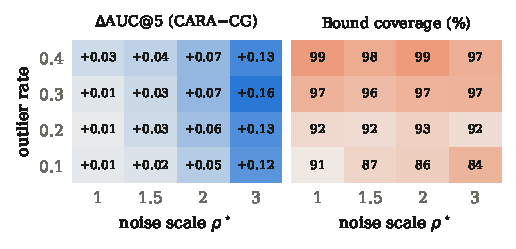
\includegraphics[width=\linewidth]{figs/grid.pdf}
\caption{Robustness grid (3 seeds $\times$ 6 scenes per cell), calibrated at noise scale $1$ and outlier rate $0.2$. Left: AUC@5 gain over CG (blue: CARA better). Right: coverage of 90\% bounds; shading grows with the distance from 90\%.}
\label{fig:grid}
\end{figure}

\section{Robustness grid}\label{sec:grid}
\Cref{fig:grid} varies the noise scale from $1$ to $3$ and the outlier rate from $0.1$ to $0.4$, with calibration fixed at $(1, 0.2)$. CARA has higher mean AUC@5 than CG in all 16 cells (gain $+0.006$ to $+0.157$) and higher than CG-$\hat\rho$ in all 16 (gain $+0.006$ to $+0.042$), and its catastrophic rate is at most that of CG in every cell except one ($1.8\%$ vs.\ $1.7\%$). Coverage depends on the outlier rate as well as on noise: when the test scenes have \emph{fewer} outliers than the calibration scenes (rate $0.1$), coverage under noise shift falls to 84--87\%, and when they have more it rises to 96--99\%. The outlier rate shifts the low quantile of cycle scores that $\hat\rho$ reads, so a change in outlier rate is partly absorbed into the drift factor. This is a second shift dimension that a scalar correction handles only approximately.


\begin{figure}[!htbp]
\centering
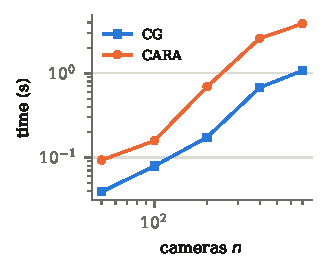
\includegraphics[width=0.55\linewidth]{figs/runtime.pdf}
\caption{Median single-thread runtime per scene (about $5.5$ edges per camera).}
\label{fig:runtime}
\end{figure}

\section{Runtime}\label{sec:runtime}
CARA costs 2--4 times as much as CG on the synthetic graphs in our implementation (\cref{fig:runtime}): $0.16$\,s vs.\ $0.08$\,s at 100 cameras and $3.9$\,s vs.\ $1.1$\,s at 700 cameras. The extra time goes to triangle scoring, the two gated solves and bridging. On the dense 715-camera Notre Dame graph (64,678 edges) the ratio is 6.2 (70\,s against 11\,s). Calibration is a one-time cost per front end and scene type (about 11\,s for 140 synthetic 100-camera scenes in a separate timing run). Triangle scoring and the Laplacian solves are standard sparse operations and would benefit from a compiled implementation.

\clearpage
\section{Development of the bound extensions}\label{sec:s5}
E1 and E2 were developed on the calibration scenes of the first ETH3D run before any test scene was used for them. Each of the 6 calibration scenes was held out in turn; thresholds were calibrated on records of the other 5 scenes and evaluated on the held-out scene, without injected failures and with 10\% or 20\% of edges replaced by random rotations (\emph{edge}) or 10\% or 20\% of cameras misread by a common rotation (\emph{camera}, see Section~\ref{sec:ext}). \Cref{tab:s5dev} shows that injected edge outliers leave the unchanged bounds near their target, while camera-level failures reduce coverage to 0.78 and hard-quarter coverage to 0.50, reproducing the pattern of the first run's test scenes. Group-conditional thresholds restore coverage in all injected conditions, and the learned normalizer with three groups (the configuration pre-registered as E2) gives the most uniform result. This prototype fixed the group boundaries on the calibration records; the released implementation fixes them on $\mathcal{D}_{\mathrm{fit}}$ as in Corollary~\ref{cor:group}. \Cref{tab:s5run1} reports the five variants on the first run's test scenes, which had been seen in aggregate before this development; the confirmatory evaluation is the second run in the main paper.

\begin{table}[!htbp]\centering\footnotesize
\caption{Development of E1/E2 on the first run's calibration scenes (leave-one-scene-out over 6 scenes, 24 sub-scenes each) with injected failures. Entries: coverage / coverage on the quarter with the largest $u_i$ / median bound width in degrees. Target 0.9.}\label{tab:s5dev}
\begin{adjustbox}{max width=\textwidth}\begin{tabular}{lccccc}\toprule
Normalizer and calibration & none & edge 10\% & edge 20\% & camera 10\% & camera 20\% \\\midrule
$u$ (unchanged) & 0.907 / 0.816 / 3.6 & 0.900 / 0.799 / 5.4 & 0.908 / 0.819 / 9.4 & 0.827 / 0.614 / 4.5 & 0.780 / 0.496 / 5.9 \\
learned $v$, augmented & 0.918 / 0.862 / 5.5 & 0.912 / 0.843 / 8.5 & 0.916 / 0.859 / 17.2 & 0.872 / 0.735 / 7.7 & 0.842 / 0.698 / 11.0 \\
$u$, 3 groups & 0.890 / 0.839 / 24.5 & 0.910 / 0.857 / 67.2 & 0.931 / 0.883 / 143.3 & 0.870 / 0.770 / 46.9 & 0.888 / 0.792 / 82.3 \\
learned $v$, 3 groups (E2) & 0.911 / 0.892 / 16.9 & 0.935 / 0.920 / 38.5 & 0.960 / 0.947 / 97.6 & 0.904 / 0.875 / 28.5 & 0.917 / 0.886 / 47.1 \\
learned $v$, augmented, 3 groups & 0.885 / 0.871 / 9.0 & 0.912 / 0.896 / 22.2 & 0.932 / 0.925 / 61.9 & 0.903 / 0.903 / 19.5 & 0.932 / 0.937 / 32.4 \\
\bottomrule\end{tabular}\end{adjustbox}\end{table}

\begin{table}[!htbp]\centering\footnotesize
\caption{Bound variants on the first ETH3D run (7 test scenes, degraded conditions pooled; these test scenes had been seen in aggregate before E1/E2 were designed). Columns as in the main paper's Table~\ref{tab:v2bounds}; E1+E2a is E1 with the learned normalizer but without groups.}\label{tab:s5run1}
\begin{tabular}{lccccc}\toprule
Variant & cov. & hard & width$^\circ$ & flagged & cat.\ flagged \\\midrule
base & 0.827 & 0.708 & 7.0 & 0.132 & 0.176 \\
E1 & 0.854 & 0.754 & 13.1 & 0.203 & 0.320 \\
E2 & 0.863 & 0.845 & 3.4 & 0.279 & 0.596 \\
E1+E2a & 0.834 & 0.770 & 5.8 & 0.119 & 0.398 \\
E1+E2 & 0.827 & 0.829 & 3.3 & 0.272 & 0.693 \\
\bottomrule\end{tabular}\end{table}


\section{Bound extensions on synthetic scenes}\label{sec:s6}
\Cref{tab:s6synth} applies the variants to the synthetic conditions of the main study. Without camera-level failures, E2 changes coverage and width little, except on sparse graphs, where it lowers coverage (0.726 against 0.767). E1 raises coverage by 1 to 5 points with about 10\% wider bounds. Combining the augmentation with group-conditional thresholds produces very wide bounds and many flags under noise shift, because the augmented failures dominate the threshold of the hardest group.

\begin{table}[!htbp]\centering\footnotesize
\caption{Bound variants on the synthetic conditions of the main study (5 seeds $\times$ 10 scenes per condition). Entries: coverage / hard-quarter coverage / median width in degrees / fraction flagged. E1+E2a is E1 with the learned normalizer but without groups.}\label{tab:s6synth}
\begin{adjustbox}{max width=\textwidth}\begin{tabular}{lccccc}\toprule
Condition & base & E1 & E2 & E1+E2a & E1+E2 \\\midrule
clean & 0.926 / 0.920 / 1.5 / 0.00 & 0.961 / 0.961 / 1.7 / 0.00 & 0.927 / 0.911 / 1.5 / 0.00 & 0.973 / 0.983 / 2.4 / 0.00 & 0.956 / 0.950 / 1.8 / 0.07 \\
fog2x & 0.915 / 0.918 / 2.9 / 0.00 & 0.947 / 0.950 / 3.3 / 0.00 & 0.904 / 0.908 / 2.9 / 0.00 & 0.972 / 0.988 / 4.8 / 0.00 & 0.908 / 0.968 / 26.0 / 0.39 \\
heavy3x & 0.970 / 0.960 / 6.5 / 0.00 & 0.983 / 0.969 / 7.2 / 0.00 & 0.957 / 0.951 / 6.0 / 0.00 & 0.956 / 0.978 / 8.0 / 0.03 & 0.949 / 0.991 / 43.2 / 0.75 \\
sparse & 0.767 / 0.778 / 3.8 / 0.00 & 0.818 / 0.817 / 4.3 / 0.00 & 0.726 / 0.744 / 3.6 / 0.00 & 0.745 / 0.803 / 4.7 / 0.03 & 0.704 / 0.832 / 25.1 / 0.41 \\
corrflip & 0.917 / 0.921 / 1.5 / 0.00 & 0.955 / 0.954 / 1.6 / 0.00 & 0.922 / 0.917 / 1.5 / 0.00 & 0.971 / 0.985 / 2.4 / 0.00 & 0.957 / 0.960 / 1.8 / 0.08 \\
large & 0.933 / 0.946 / 2.5 / 0.00 & 0.965 / 0.973 / 2.7 / 0.00 & 0.918 / 0.933 / 2.4 / 0.00 & 0.964 / 0.986 / 3.7 / 0.00 & 0.895 / 0.943 / 13.3 / 0.24 \\
\bottomrule\end{tabular}\end{adjustbox}\end{table}


\clearpage
\section{Pre-registration file}\label{sec:s7}
The pre-registration for the confirmatory run, reproduced verbatim from the released repository (file \texttt{experiments/ext/PREREGISTRATION.md}). The first two parts were written on 26 September 2026 before the run-2 outputs were computed; the note on the secondary variant E2u was added the same day, also before any run-2 output existed.

{\footnotesize
\begin{Verbatim}[breaklines=true]
# Pre-registration for ETH3D run 2 (written 2026-09-26, before run 2 data exist)

Run 2 (`out_eth3d_v2`, seed 3, new sub-scenes, all 13 scenes, leave-one-scene-out calibration) is the
confirmatory test for the bound extensions. Everything below was fixed after looking at run 1 results.

Design history (disclosed in the paper):
- E1 (failure-mode augmentation) and E2 (learned normalizer, group-conditional thresholds) were designed on
  ETH3D *calibration* scenes with injected failures (leave-one-scene-out), see `dev_eth3d.py`, `dev_eval.py`.
- The five variants in `eval_bounds.py` were then evaluated on run 1 test scenes, which had been seen in
  aggregate before. On run 1, E2 without augmentation gave the best coverage on hard cameras.

Primary hypotheses for run 2 (one-sided, unit = test scene, exact sign-flip test, Holm over H1-H3):
- H1: E2 raises coverage over base on the hardest quarter of cameras (by u), pooled over the 6 degraded conditions.
- H2: E2 raises overall coverage over base, pooled over the 6 degraded conditions.
- H3: E2's normalizer ranks catastrophic cameras (error > 30 deg) better than u (per-scene AUROC, pooled).
Secondary: all five variants reported; width among unflagged cameras; flag rate; clean coverage.
Primary variant: E2 = Config(cam_norm="learn", cam_groups=3), alpha_cam = 0.1, calibrated on clean scenes.
No setting is changed after run 2 results are seen.

## Additional run-2 hypotheses (E3, E5), fixed before run 2 data exist
- E3 features and model: `cara/edge_uncertainty.py` (f1-f5, linear model for log error, fitted on the D_fit split).
- H4: CARA with the learned sigma has higher AUC@5 than CARA with the pre-registered sigma (f1), pooled over all 7 conditions.
- H5: outlier-edge AUROC (error > 5 deg) of the learned sigma exceeds that of f1 (per scene, pooled).
- E5 (`cara/translation.py`): LUD translation averaging on VGGT relative translations, rotated by each method's
  global rotations, all edges; CARA additionally with only its accepted edges ("CARA+gate").
- H6: CARA+gate has lower median scale-free position error than CG (all edges), pooled over conditions.
Unit of inference: test scene (13 scenes, leave-one-scene-out calibration), exact sign-flip test; Holm over H1-H6.

## Note added after the run-1 per-camera analysis (still before run 2 data exist)
On run 1, the learned normalizer did not rank catastrophic cameras better than u (AUROC 0.81-0.90 for u), so H3 is
expected to fail; E2's coverage gain comes from the group-conditional thresholds. A secondary variant E2u
(groups on u, no learned normalizer) is added to `eval_bounds.py`. H1-H6 and the primary variant are unchanged.

\end{Verbatim}
}

\bibliographystyle{elsarticle-num}
\bibliography{refs}
\end{document}
